\subsection{Graphing with Derivatives}

\subsubsection{Maxima and Minima}
One helpful application of derivatives is to determine the maximum and minimum values of a function.\\
\\
Definitions:
\begin{itemize}
    \item Local maximums are the highest values of the function in relation to the surrounding points.
    \item Local minimums are the lowest values of the function in relation to the surrounding points.
    \item Absolute/Global maximums are the highest value(s) of the function defined on a closed interval $[a,b]$.
    \item Absolute/Global minimums are the lowest value(s) of the function defined on a closed interval $[a,b]$.
\end{itemize}
Local max/mins can be found at any of the three locations:
\begin{itemize}
    \item Critical Points:\\
    where the derivative is equal to zero.
    \item Boundary Points:\\
    the limits of where the function is defined. i.e. if the function were defined over $[a,b]$, then $a$ and $b$ would be boundary points.\\
    This also extends to places the where the function is undefined.
    \item Singular Points/Cusps:\\
    places where the derivative is undefined. i.e. for $y=|x|$, a singular point would be located at $(0,0)$
\end{itemize}
Ex: $y=x^2$ over $(-\infty,\infty)$ has an absolute minimum at $(0,0)$ and no absolute maximum.\\
However, $y=x^2$ over $[-2,2]$ has an absolute minimum at $(0,0)$ and absolute maximums at $(-2,4)$ and $(2,4)$.\\
\\
Calculating Critical Points:\\
If $c$ is a critical point of $f$, then $f'(c)=0$.\\
Ex: Find critical points of $y=3x^4-4x^3$.
\begin{align*}
    &y'=12x^3-12x^2=0\\
    &0=12x^2(x-1)\\
    &x=0,\,x=1
\end{align*}
\\
Second Derivative Test:\\
We can determine if a critical point is a minimum, maximum, or inflection point by the 2nd derivative test:
\begin{align*}
    \text{For where }c\text{ is a critical point, }
    &\text{If }f''(c)<0\text{, then $f$ has a local maximum at $x=c$}\\
    &\text{If }f''(c)>0\text{, then $f$ has a local minimum at $x=c$}\\
    &\text{If }f''(c)=0\text{, then $f$ has a point of inflection at $x=c$}
\end{align*}
Ex: Determine local max/mins of $y=3x^4-4x^3$
\begin{align*}
    &f'(x)=12x^3-12x^2\\
    &f''(x)=36x^2-24x\\
    &\text{Critical Points: }\\
    &12x^3-12x^2=0\Ra x=0,\,x=1\\
    &\text{2nd Derivative Test:}\\
    &f''(0)=36(0)^2-24(0)=0\\
    &\therefore x=0\text{ is an inflection point}\\
    &f''(1)=36(1)^2-24(1)=12>0\\
    &\therefore x=1\text{ is a local minimum}
\end{align*}

\subsubsection{Mean Value Theorem}
Rolle's Theorem:\\
If $y=f(x)$ is continuous on $[a,b]$ and is differentiable on $(a,b)$ and if $f(a)=f(b)=0$ then there is at least one point $c$ between $a$ and $b$ at which $f'(c)=0$.\\
Loosely speaking, what comes up must come down.\\
\centerline{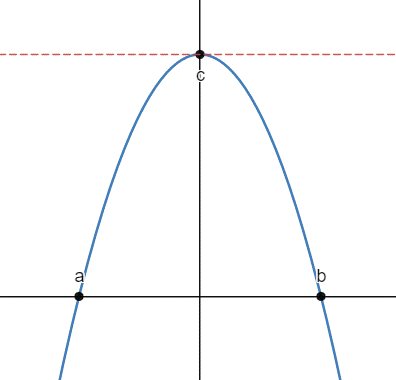
\includegraphics[scale=0.6]{DifferentialCalculusPictures/RollesTheorem.png}}

Intermediate Value Theorem:\\
If $f(x)$ is continuous on $[a,b]$ then there exists some real number $f(c)$ between $f(a)$ and $f(b)$ such that $a<c<b$\\
Ex: Show that there exists a positive real number $0<x<\frac{\pi}{2}$ for which $\cos(2x)=\sin x$
\begin{align*}
    &f(x)=\cos 2x-\sin x\\
    &f(0)=1\\
    &f\brround{\frac{\pi}{2}}=-2
\end{align*}
By the IVT, this guarantees that $f(x)$ must have at least one solution because the function must cross the x-axis.\\
Ex2: Find a solution to $f(x)=x^5-2x^4+2$
\begin{align*}
    &\lim_{x\to\infty}f(x)=\infty\text{ and }\lim_{x\to-\infty}f(x)=-\infty\therefore\text{ a solution exists}\\
    &f(-1)=-1,\,f(0)=2,\,f(1)=1
\end{align*}
By IVT, there is a zero between $-1$ and 0.\\
Using bisection, we can approximate the solution through multiple iterations.
\begin{align*}
    &-1<x<0\\
    &f\brround{-\frac{1}{2}}>0\therefore\,-1<x<-\frac{1}{2}\\
    &f\brround{-\frac{3}{4}}>0\therefore\,-1<x<-\frac{3}{4}\\
    &\vdots\\
    &-0.9104728699\ldots<x<-0.9104719162\ldots
\end{align*}
\\
Mean Value Theorem:\\
Rolle's Theorem is a generalization of the Mean Value Theorem (MVT). The MVT states that if $y=f(x)$ is a continuous function over $[a,b]$ and is differentiable on $(a,b)$ then there is at least one number $c$ between $a$ and $b$ such that:
$$\frac{f(b)-f(a)}{b-a}=f'(c)$$
Essentially, if you take the average between two points, a continuous function must attain that average value at least once.\\
\centerline{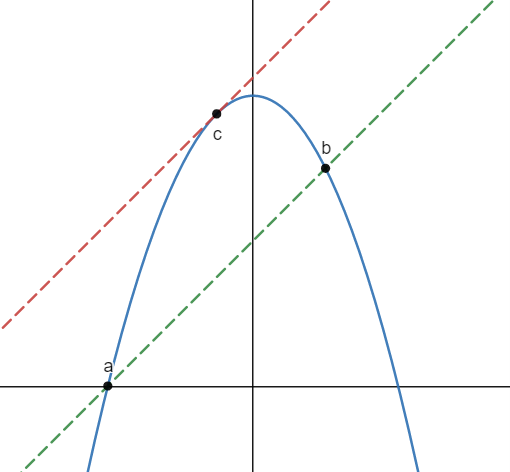
\includegraphics[scale=0.6]{DifferentialCalculusPictures/MVTImage.png}}
Ex: for the function $\frac{1}{x}$ over $[1,3]$ find all values $c$ that satisfy the mean value theorem.
\begin{align*}
    &f(x)=\frac{1}{x}\\
    &f'(x)=-\frac{1}{x^2}\\
    &f'(c)=\frac{f(3)-f(1)}{3-1}\\
    &-\frac{1}{c^2}=\frac{\frac{1}{3}-1}{2}=\frac{-\frac{2}{3}}{2}=-\frac{1}{3}\\
    &\Ra c^2=3\\
    &c=\pm\sqrt{3}\\
    &\text{Check domain } c\in(1,3)\\
    &c=\sqrt{3}
\end{align*}
Ex2: Show that for $0<x<\frac{\pi}{2}$, $\tan x<x$
\begin{align*}
    &f(x)=\tan x,\,f'(x)=\sec^2x\\
    &\frac{f(x)-f(a)}{x-a}=f'(c)\Ra f(x)=f(a)+f'(c)(x-a)\\
    &\text{set }a=0\\
    &f(x)=\tan x=\sec^2c\cdot x\\
    &\text{recall }0<c<\frac{\pi}{2}\therefore \sec c>0\\
    &\Ra\tan x=\sec^2c\cdot x>x\\
    &\therefore\tan x>x
\end{align*}
Ex3: Suppose $1\leq f'(t)\leq 5$ for all $t$ and $f(0)=0$. What are possible values of $t$ for which $f(t)=3000$?
\begin{align*}
    &\frac{f(t)-0}{t-0}=\frac{3000}{t}=f'(c)\text{ for }1\leq f'(c)\leq 5\\
    &1\leq\frac{3000}{t}\leq 5\\
    &\frac{1}{5}\leq\frac{t}{3000}\leq 1\\
    &600\leq t\leq 3000
\end{align*}
Ex4: Show that $|\sin x-\sin y|\leq |x-y|$ for all $x,y$
\begin{align*}
    &f(t)=\sin t,\,f'(t)=\cos t\\
    &\frac{\sin x-\sin y}{x-y}=\cos c\\
    &\left|\frac{\sin x-\sin y}{x-y}\right|=|\cos c|\leq 1\\
    &\therefore\,|\sin x-\sin y|\leq |x-y|
\end{align*}

\subsubsection{L'H\^opital's Rule}
L'H\^opital's Rule states that: Provided the limit exists, if $f(x_0)=g(x_0)=0$ then:
$$\lim_{x\to x_0}\frac{f(x)}{g(x)}=\lim_{x\to x_0}\frac{f'(x)}{g'(x)}$$
This allows us to calculate limits with indeterminate forms such as $\frac{0}{0}$.\\
Indeterminate forms can be any of the following:
\begin{align*}
    &\frac{0}{0}\\
    &\frac{\infty}{\infty}\\
    &0\cdot\infty\\
    &0^0\\
    &\infty^0\\
    &1^\infty\\
    &\infty-\infty
\end{align*}
\begin{align*}
    \text{Ex: }&\lim_{x\to 1}\frac{x^3-x^2-x+1}{x^3-2x^2+1}\\
    &=\lim_{x\to 1}\frac{3x^2-2x-1}{3x^2-4x+1}=\frac{0}{0}\\
    &=\lim_{x\to 1}\frac{6x-2}{6x-4}\\
    &=2
\end{align*}
Solving for $\frac{0}{0}$ and $\frac{\infty}{\infty}$ is easy as they are already in fraction form. The other indeterminate forms are trickier to solve.\\
For $0\cdot\infty$ we can rewrite it in the form of
    $$\lim_{x\to a}f(x)g(x)=\lim_{x\to a}\frac{f(x)}{1/g(x)}$$
\begin{align*}
    \text{Ex: }&\lim_{x\to 0^+}x^2\ln x\\
    &=\lim_{x\to 0^+}\frac{\ln x}{1/x^2}=\frac{-\infty}{\infty}\\
    &=\lim_{x\to 0^+}\frac{1/x}{-2/x^3}=-\frac{1}{2}\lim_{x\to 0^+}x^2\\
    &=0
\end{align*}
For any limits with exponentials we can take the log of both sides and solve for the log of the limit and then exponentiate to get the limit.
\begin{align*}
    \lim_{x\to a}f(x)^{g(x)}\\
    \Ra\lim_{x\to a}g(x)\ln(f(x))=L\\
    \lim_{x\to a}f(x)^{g(x)}=e^L
\end{align*}
\begin{align*}
    \text{Ex: }&\lim_{x\to 0^+}\brround{\frac{1}{\sin x}}^{\sin x}\\
    &\lim_{x\to 0^+}-\sin x\ln(\sin x)=L\\
    &L=\lim_{x\to 0^+}\frac{\ln(\sin x)}{1/\sin x}=\lim_{x\to 0^+}\frac{\ln(\sin x)}{\csc x}\\
    &L=\lim_{x\to 0^+}\frac{\frac{\cos x}{\sin x}}{-\csc x\cot x}=\lim_{x\to 0^+}\brround{-\sin x}=0\\
    &\therefore \lim_{x\to 0^+}\brround{\frac{1}{\sin x}}^{\sin x}=e^0=1
\end{align*}
\begin{align*}
    \text{Ex2: }&\lim_{x\to \infty}\brround{1+\frac{a}{x}}^{bx}\\
    &L=\lim_{x\to \infty}bx\ln\brround{1+\frac{a}{x}}=\lim_{x\to \infty}\frac{b\ln\brround{1+\frac{1}{a}}}{1/x}=\lim_{x\to \infty}\frac{b\brround{\frac{1}{1+\frac{a}{x}}}\brround{\frac{-a}{x^2}}}{\frac{-1}{x^2}}\\
    &=\lim_{x\to \infty}\frac{ab}{1+\frac{a}{x}}=ab\\
    &\therefore \lim_{x\to \infty}\brround{1+\frac{a}{x}}^{bx}=e^{ab}
\end{align*}

\subsubsection{Curve Sketching}
The derivative of a function is a powerful tool in being able to graph it.\\
First Derivative Test:
\begin{itemize}
    \item If $f'(x)>0$ over $(a,b)$ then $f(x)$ is increasing on $[a,b]$
    \item If $f'(x)<0$ over $(a,b)$ then $f(x)$ is decreasing on $[a,b]$
    \item If $f'(x)=0$ then $f(x)$ will have a local max/min
\end{itemize}
To see what the curve of the graph looks like we can use the concavity:\\
\centerline{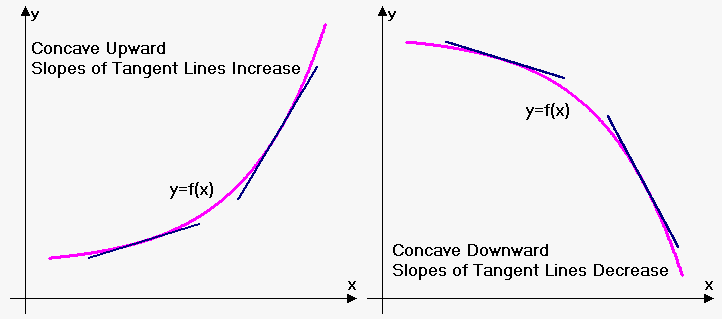
\includegraphics[scale=0.7]{DifferentialCalculusPictures/Concavity.png}}
The point where a curve changes concavity is called an inflection point.\\
Second Derivative Test:
\begin{itemize}
    \item If $f''(x)>0$ over $(a,b)$ then $f(x)$ is concave up.
    \item If $f''(x)<0$ over $(a,b)$ then $f(x)$ is concave down.
    \item If $f''(x)=0$ then $f(x)$ will have an inflection point.
\end{itemize}
Many functions can be simplified by exposing some symmetry:
\begin{description}
    \item[Even Function:] A function is even if $f(-x)=f(x)$.\\
    This means that all points are reflected across the y-axis.\\
    Ex: $y=\cos x$ or $y=x^2$
    \item[Odd Function:] A function is odd if $f(-x)=-f(x)$\\
    This means that the function is symmetric across the origin.\\
    Ex: $y=\sin x$ or $y=x^3$
\end{description}
The last thing yet to consider is what happens at the end points and asymptotes of a function.\\
We want to take the limit of the function at $\pm\infty$ and any points where the function is undefined to find any potential asymptotes.\\
Oblique asymptotes may occur in rational functions where the degree of the numerator is one higher than the degree in the denominator.
\begin{align*}
    \text{Ex: }&y=\dfrac{x^2-16}{x-7}\\
    &\text{by long division }\frac{x^2-16}{x-7}=x+7+\frac{33}{x-7}
\end{align*}
As $|x|$ gets very large, the $\dfrac{33}{x-7}$ term tends to 0 so $f(x)$ approaches the function $y=x+7$ as $|x|$ gets very large.\\
Put all together, we can follow a general procedure to sketch curves.
\begin{enumerate}
    \item Identify the base function and expected behavior
    \item Find the domain (and range) of the function and any non permissible values
    \item Identify any symmetry
    \item Plot any known intercepts
    \item Find all asymptotes and end behavior
    \item Find critical points
    \item First derivative test
    \item Find inflection points
    \item Second derivative test
\end{enumerate}
Ex: $y=\dfrac{x}{\ln x}$\\
Domain: $x>0$\\
NPVs: $x\neq 0$, $x\neq 1$\\
Symmetry: none\\
Intercepts: none\\
Asymptotes and boundaries:
\begin{align*}
    &\lim_{x\to 0^+}\frac{x}{\ln x}=\frac{0}{-\infty}=0\\
    &\lim_{x\to 1^-}=\frac{1}{0^-}=-\infty\\
    &\lim_{x\to 1^+}=\frac{1}{0^+}=\infty\\
    &\lim_{x\to \infty}=\infty
\end{align*}
Critical Points:
\begin{align*}
    &f'(x)=\frac{\ln x-x\brround{\frac{1}{x}}}{(\ln x)^2}=\frac{\ln x-1}{(\ln x)^2}\\
    &f'(x)=0\Ra \ln x=1\\
    &x=e\\
    &f(e)=e\\
    &\rightarrow (e,e)
\end{align*}
First Derivative Test:\\
\begin{tabular}{c||c|c}
    Interval & $f'(x)$ & $f(x)$\\
    \hline
    $0<x<1$ & $-$ & decreasing\\
    $1<x<e$ & $-$ & decreasing\\
    $x>e$ & $+$ & increasing
\end{tabular}\\
Inflection Points:
\begin{align*}
    &f''(x)=\frac{2-\ln x}{x(\ln x)^3}\\
    &f''(x)=0\Ra \ln x=2\\
    &x=e^2\\
    &f(e^2)=\frac{e^2}{2}\\
    &\rightarrow \brround{e^2,\frac{e^2}{2}}
\end{align*}
Second Derivative Test:\\
\begin{tabular}{c||c|c}
    Interval & $f''(x)$ & $f(x)$\\
    \hline
    $0<x<1$ & $-$ & concave down\\
    $1<x<e^2$ & $+$ & concave up\\
    $x>e^2$ & $-$ & concave down
\end{tabular}\\
\\
\centerline{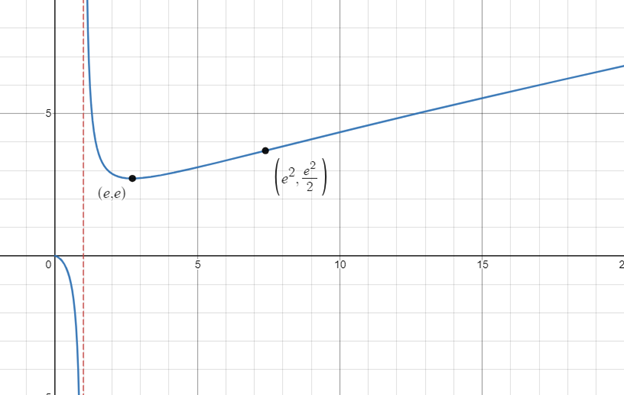
\includegraphics[scale=0.9]{DifferentialCalculusPictures/SketchingEx1.png}}
